\section{ECC2K-130 on FPGA}
\label{sec:ecc2k-fpga}

Two FPGA designs, two measurements, one field. This library's core is
a digit-serial walker that simulates with open tools and reports area
in yosys LUT4; it has no vendor place-and-route, so it has no
iterations-per-second figure. The companion engine is a pipelined
Karatsuba walker measured on an AWS F2. They are not the same number
in different units.

\subsection{Digit-serial core}
\label{sec:fpga-core}

\texttt{fpga/rtl/ecc2k130\_step.v} walks $R\leftarrow\sigma^j(R)+R$
with one multiplier per core, Itoh--Tsujii over that multiplier, and
back-pressure that stops the walk rather than dropping a point. The
collector is round-robin: a starved core stops walking, so a
fixed-priority arbiter would quietly reduce a fleet of cores to one.
Table~\ref{tab:fpga-cycles} is Icarus Verilog, cycles per operation,
every row's RTL having passed the full vector comparison against the
golden model.\art{fpga/README.md, ``Numbers''}

\begin{table}[t]
\centering
\small
\caption{Digit-serial ONB core, Icarus Verilog. Area is yosys mapped
  to 4-input LUTs, not a placed-and-routed device figure. No fmax, so
  no iterations/s.}
\label{tab:fpga-cycles}
\begin{tabular}{@{}rrrrr@{}}
\toprule
DIGIT & cyc/mul & cyc/inv & cyc/step & LUT4 (1 core) \\
\midrule
1 & 132 & --- & 1\,342 & 7\,301 \\
2 & 67 & --- & 692 & 7\,561 \\
4 & 34 & 289 & \textbf{362} & \textbf{7\,941} \\
8 & 18 & --- & 202 & 8\,607 \\
16 & 10 & --- & 122 & 10\,045 \\
\bottomrule
\end{tabular}
\end{table}

Two and four cores at DIGIT${}=4$ map to $15{,}705$ and $31{,}437$
LUT4: cores scale linearly, they share nothing. From DIGIT 1 to 16
the cycles per step fall $11\times$ while the area grows $1.38\times$,
so the area--time product improves about $8\times$, with the caveat
that a wider digit lengthens the combinational path and only vendor
timing analysis says whether the clock survives it.

What is deliberately not quoted: iterations per second, points per
day, ``break time'', or a comparison against the GPU. All of those
need an fmax this flow cannot produce. The host tool
\texttt{fpga/host/ec2k} starts, walks, verifies and merges
distinguished-point files; \texttt{verify} replays every point the
board reported against the golden model.

\subsection{Companion engine on F2}
\label{sec:fpga-f2}

The companion VHDL engine uses a pipelined Karatsuba multiplier in
the same permuted type-II basis, a step unit that shares one inversion
across a batch of walks ($5+5/W$ multiplies per step), and a sequencer
that reports distinguished points. Testbenches are checked against
the client's field model. On an AWS \texttt{f2.6xlarge} (VU47P):

\begin{center}
\small
\begin{tabular}{@{}lrr@{}}
\toprule
image & clocks/step & G steps/s \\
\midrule
48 engines & 5.31 & 3.01 \\
64 engines & 5.31 & 4.01 \\
80 engines & 5.31 & 5.02 \\
96 engines, 333~MHz & 5.31 & 6.02 \\
112 engines, 375~MHz & --- & 8.12 \\
\textbf{128 engines, 333~MHz} & \textbf{5.17} & \textbf{8.25} \\
120 engines, 333~MHz & --- & 7.73 \\
\bottomrule
\end{tabular}
\end{center}

The 128-engine image at 333~MHz holds $8{,}249$~M steps/s, i.e.\
$8.25$~G steps/s, with distinguished points sampled from each engine
checked against the client's reference walk and no drops in the listed
run.\art{crypto:hdl/ecc2k130/README.md}\art{crypto:hdl/ecc2k130/aws/README.md}
Figure~\ref{fig:fpga} draws the measured F2 images against engine
count. The engineering estimate before the board was $5$--$12$~B/s per
VU47P, central estimate about $8$~B/s; the measurement landed on that
central estimate and is a device number, not the estimate
reprised.\art{crypto:ecc2k130/FPGA-CEILING.md}

\begin{figure}[t]
\centering
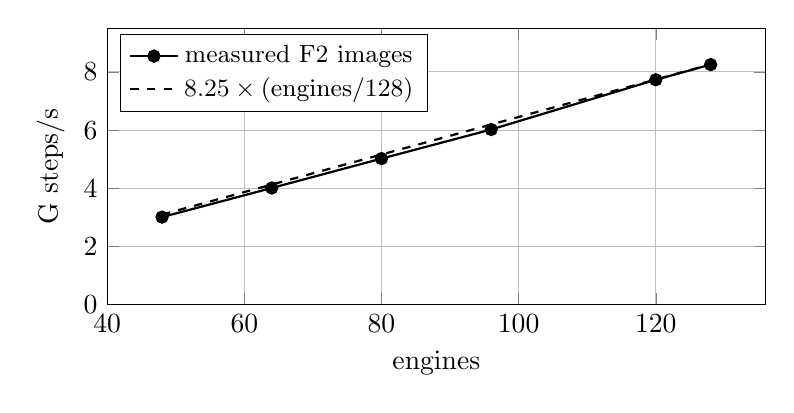
\begin{tikzpicture}
\begin{axis}[
  width=0.82\textwidth,
  height=0.42\textwidth,
  xlabel={engines},
  ylabel={G steps/s},
  xmin=40, xmax=136,
  ymin=0, ymax=9.5,
  grid=major,
  legend style={at={(0.02,0.98)},anchor=north west,font=\small},
]
\addplot[mark=*,thick] coordinates {
  (48,3.01) (64,4.01) (80,5.02) (96,6.02) (120,7.73) (128,8.25)
};
\addlegendentry{measured F2 images}
\addplot[dashed,domain=48:128,thick] {0.0645*x};
\addlegendentry{$8.25\times(\mathrm{engines}/128)$}
\end{axis}
\end{tikzpicture}
\caption{Companion ECC2K-130 FPGA engine on AWS F2. The 128-engine
  image at $333$~MHz is $8.25$~G steps/s. Linear scaling with engine
  count is the prediction of a design that shares nothing between
  engines except the host port. This library's digit-serial core is
  not on this figure: it has no fmax.}
\label{fig:fpga}
\end{figure}

FPGA workers speak the same client contract as the GPUs and write the
same 32-byte records, so a collision between an FPGA trail and a GPU
trail is an ordinary merge.
